% Copyright 2011-2019 David Hadka.  All Rights Reserved.
%
% This file is part of the MOEA Framework User Manual.
%
% Permission is granted to copy, distribute and/or modify this document under
% the terms of the GNU Free Documentation License, Version 1.3 or any later
% version published by the Free Software Foundation; with the Invariant Section
% being the section entitled "Preface", no Front-Cover Texts, and no Back-Cover
% Texts.  A copy of the license is included in the section entitled "GNU Free
% Documentation License".

\section{What is the MOEA Framework?}

The MOEA Framework is a free and open source Java library for developing and experimenting with multiobjective evolutionary algorithms (MOEAs) and other general-purpose optimization algorithms.  A number of algorithms are provided out-of-the-box, including NSGA-II, NSGA-III, $\epsilon$-MOEA, GDE3 and MOEA/D.  In addition, the MOEA Framework provides the tools necessary to rapidly design, develop, execute and statistically test optimization algorithms.  The following features of the MOEA Framework distinguish it from available alternatives:

\paragraph{Fast, reliable implementations of many state-of-the-art multiobjective evolutionary algorithms.}  The MOEA Framework contains internally NSGA-II, NSGA-III, $\epsilon$-MOEA, $\epsilon$-NSGA-II, PAES, PESA2, SPEA2, IBEA, SMS-EMOA, GDE3, SMPSO, OMOPSO, CMA-ES, and MOEA/D.  These algorithms are optimized for performance, making them readily available for high performance applications.  By also supporting the JMetal and PISA libraries, the MOEA Framework provides access to $30$ multiobjective optimization algorithms.

\paragraph{Extensible with custom algorithms, problems and operators.}  The MOEA Framework provides a base set of algorithms, test problems and search operators, but can also be easily extended to include additional components.  Using a Service Provider Interface (SPI), new algorithms and problems are seamlessly integrated within the MOEA Framework.  

\paragraph{Modular design for constructing new optimization algorithms from existing components.}  The well-structured, object-oriented design of the MOEA Framework library allows combining existing components to construct new optimization algorithms.  And if needed functionality is not available in the MOEA Framework, you can always extend an existing class or add new classes to support any desired feature.

\paragraph{Permissive open source license.}  The MOEA Framework is licensed under the free and open GNU Lesser General Public License, version 3 or (at your option) any later version.  This allows end users to study, modify, and distribute the MOEA Framework freely.

\paragraph{Fully documented source code.}  The source code is fully documented and is frequently updated to remain consistent with any changes.  Furthermore, an extensive user manual is provided detailing the use of the MOEA Framework in detail.

\paragraph{Extensive support available online.}  As an actively maintained project, bug fixes and new features are constantly added.  We are constantly striving to improve this product.  To aid this process, our website provides the tools to report bugs, request new features, or get answers to your questions.

\paragraph{Over 1200 test cases to ensure validity.}  Every release of the MOEA Framework undergoes extensive testing and quality control checks.  And, if any bugs are discovered that survive this testing, we will promptly fix the issues and release patches.  

\section{Which Distribution is Right for Me?}

The MOEA Framework is currently distributed in three forms: 1) the compiled binaries; 2) the source code; and 3) the demo application.  The following text describes each distribution and its intended audience.

\paragraph{Compiled Binaries}
The compiled binaries distribution contains a fully-working MOEA Framework installation.  All required third-party libraries, data files and documentation are provided.  This download is recommended for developers integrating the MOEA Framework into an existing project.

\paragraph{Source Code}
The source code distribution contains all source code, unit tests, documentation and data files.  This distribution gives users full control over the MOEA Framework, as any component can be modified as needed.  As such, this download is recommended for developers wishing to contribute to or study the inner workings of the MOEA Framework.

\paragraph{Demo Application}
The demo application provides several interactive demos of the MOEA Framework launched by double-clicking the downloaded JAR file.  This download is intended for first-time users to quickly learn about the MOEA Framework and its capabilities.

\section{Obtaining a Copy}

The various MOEA Framework distributions can be downloaded from our website at \webpage{moeaframework.org/}.  The compiled binaries and source code distributions are packaged in a compressed tar (.tar.gz) file.  Unix/Linux/Mac users can extract the file contents using the following command:

\begin{lstlisting}[language=Plaintext]
tar -xzf MOEAFramework-%VERSION%.tar.gz
\end{lstlisting}

\noindent
Windows users must use an unzip utility like 7-Zip to extract the file contents.  7-Zip is a free, open source program which can be downloaded from \webpage{http://www.7-zip.org/}.

\section{Installing Dependencies}

The software packages listed below are required or recommended in order to use the MOEA Framework.  Any software package marked as required MUST be installed on your computer in order to use the MOEA Framework.  Software marked as optional is not required to be installed, but will generally make your life easier.

\subsection{Java 6+ (Required)}
Java 6, or any later version, is required for any system running the MOEA Framework.  If downloading the compiled binaries or demo application, you only need to install the Java Runtime Environment (JRE).  The source code download requires the Java Development Kit (JDK), which contains the compiler and other developer tools.  We recommend one of the following vendors (most are free):

\begin{description}
  \item[Oracle] - \webpage{http://www.oracle.com/technetwork/java/javase/}
    \begin{itemize}
      \item For Windows, Linux and Solaris
    \end{itemize}
    
  \item[JRockit JDK] - \webpage{http://www.oracle.com/technetwork/middleware/jrockit/}
    \begin{itemize}
      \item For Windows, Linux and Solaris
      \item May provide better performance and scalability on Intel 32 and 64-bit architectures
    \end{itemize}

  \item[OpenJDK] - \webpage{http://openjdk.java.net/}
    \begin{itemize}
      \item For Ubuntu 8.04 (or later), Fedora 9 (or later), Red Hat Enterprise Linux 5, openSUSE 11.1, Debian GNU/Linux 5.0 and OpenSolaris
    \end{itemize}

  \item[IBM] - \webpage{http://www.ibm.com/developerworks/java/jdk/}
    \begin{itemize}
      \item For AIX, Linux and z/OS
    \end{itemize}
  \item[Apple] - \webpage{http://support.apple.com/kb/DL1572}
\end{description}

Please follow the installation instruction accompanying your chosen JRE or JDK.

\subsection{Eclipse or NetBeans (Optional)}
Eclipse and NetBeans are two development environments for writing, debugging, testing, and running Java programs.  Eclipse can be downloaded for free from \webpage{eclipse.org/}, and NetBeans can be obtained from \webpage{netbeans.org/}.

The installation of Eclipse is simple --- just extract the compressed file to a folder of your choice and run the Eclipse executable from this folder.  First-time users of Eclipse may be prompted to select a workspace location.  The default location is typically fine.  Click the checkbox to no longer show this dialog and click Ok.

To install NetBeans, simply run the downloaded executable.  Once installed, you can launch NetBeans by clicking the NetBeans link in your start menu.

\subsection{Apache Ant (Optional)}
Apache Ant is a Java tool for automatically compiling and packaging projects, similar to the Make utility on Unix/Linux.  Individuals working with the source code distribution should consider installing Apache Ant, as it helps automate building and testing the MOEA Framework.  Apache Ant can be downloaded from \webpage{http://ant.apache.org/}.  The installation instructions provided by Ant should be followed.

Note that Eclipse contains Ant, so it is not necessary to install Eclipse and Ant together.

\section{Importing into Eclipse}
When working with the source code distribution, it is necessary to properly configure the Java environment to ensure all resources are available.  To assist in this process, the source code distribution includes the necessary files to import directly into Eclipse.

To import the MOEA Framework project into Eclipse, first start Eclipse and select File $\rightarrow$ Import... from the menu.  A popup window will appear.  Ensure the General $\rightarrow$ Existing Projects into Workspace item is selected and click Next.  A new window will appear.  In this new window, locate the Set Root Directory entry.  Using the Browse button, select the \folder{\moeaframework} folder.  Finally, click Finish.  The MOEA Framework will now be properly configured in Eclipse.

\section{Importing into NetBeans}
If you downloaded the source code, you can import the MOEA Framework into NetBeans as follows.  In NetBeans, select New Project from the File menu.  In the screen that appears, select the ``Java'' category and ``Java Project with Existing Sources''.  Click Next.

Specify the project name as ``MOEA Framework''.  Set the project folder by clicking the Browse button and selecting the \folder{\moeaframework} folder.  Click Next.

Add the \folder{src} and \folder{examples} folders as Source Package Folders.  Click Finish.  The MOEA Framework project should now appear in the Projects window.

Finally, we need to add the third-party libraries used by the MOEA Framework.  Right-click the MOEA Framework project in the Projects window and select Properties.  In the window that appears, click Libraries in the left-hand panel.  On the right-side of the window, click the button ``Add Jars/Folder''.  Browse to the \folder{\moeaframework/lib} folder, highlight all the JAR files (using shift or alt to select multiple files), and click Ok.  Be sure that you select each individual JAR file and not the folder containing the JAR files.  Click the ``Add Jars/Folder'' button again.  Navigate to and select the root \folder{\moeaframework} folder, and click Ok.  You should now see $8$ items in the compile-time libraries list.  There should be $7$ entries referencing \plaintext{.jar} files the ``\folder{.}'' as the last entry.  Your screen should look like the figure below.  Click Ok when finished.

%\begin{figure}
\begin{center}
  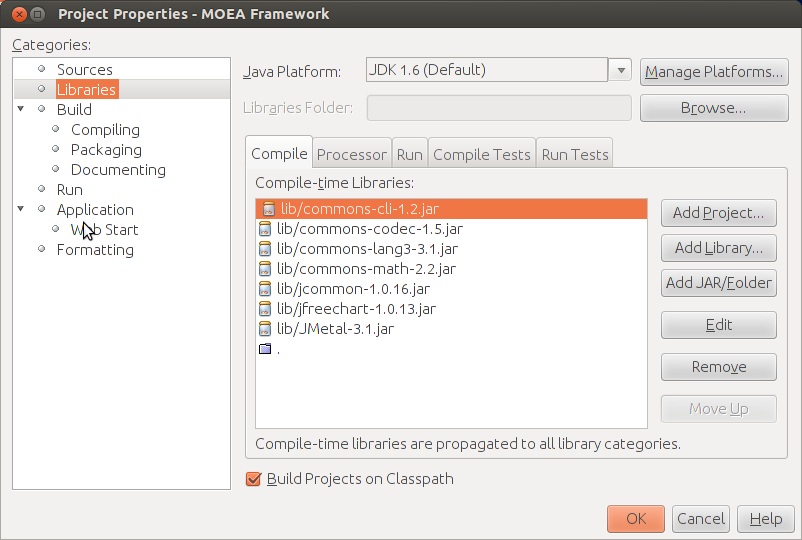
\includegraphics[width=.6\linewidth]{netbeans.png}
\end{center}
%  \caption{How the NetBeans properties window should appear in the MOEA Framework is properly configured.}
%  \label{fig:netbeans}
%\end{figure}

Test your NetBeans install by running Example1.  You can run an example by expanding the \folder{examples} folder in the Project window, right-clicking Example1, and selecting Run File from the popup menu.

\section{Resolving Dependencies with Maven}
Since version 2.4, the MOEA Framework and its dependencies can be resolved using the Maven dependency management system.  Maven is available from \webpage{http://maven.apache.org/}.  To add the MOEA Framework to your Maven project, add the following dependency to your \file{pom.xml} file:

\begin{lstlisting}[language=Plaintext]
<dependency>
	<groupId>org.moeaframework</groupId>
	<artifactId>moeaframework</artifactId>
	<version>%VERSION%</version>
</dependency>
\end{lstlisting}

If this is your first time using Maven, check out the Maven in 5 Minutes guide at \webpage{http://maven.apache.org/guides/getting-started/maven-in-five-minutes.html}.

\section{Testing your Installation}
Having finished installing the MOEA Framework and its dependencies, it is useful to run the MOEA Diagnostic Tool to test if the installation was successful.  If the diagnostic tool appears and you can run any algorithm, then the installation was successful.

\paragraph{Compiled Binaries}
Run the launch-diagnostic-tool.bat file on Windows.  You can manually run the diagnostic tool with the following command:

\begin{lstlisting}[language=Plaintext]
java -Djava.ext.dirs=lib
		org.moeaframework.analysis.diagnostics.LaunchDiagnosticTool
\end{lstlisting}

\paragraph{Source Code}
Inside Eclipse, navigate to the src $\rightarrow$ org $\rightarrow$ moeaframework $\rightarrow$ analysis $\rightarrow$ diagnostic package in the Package Explorer window.  Right-click the file \texttt{LaunchDiagnosticTool.java} and select the Run as $\rightarrow$ Java Application option in the popup menu.

\paragraph{Demo Program}
Double-click the downloaded JAR file.  If the demo window does not appear, try to manually launch the tool with with the following command:

\begin{lstlisting}[language=Plaintext]
java -jar MOEAFramework-%VERSION%-Demo.jar
\end{lstlisting}

\section{Running Examples}
Several example applications are provided with the MOEA Framework in the \folder{\moeaframework/examples/} folder.  If using Eclipse or Netbeans, you can run these examples directly within the GUI.  For example, in Eclipse, right-click Example1.java and select Run as $\rightarrow$ Java Application.  If running from the command line, you will first need to compile the code using the Java compiler (\texttt{javac}) followed by running the example in the Java virtual machine (\texttt{java}).  For example, you can compile and run the first example on Windows as follows:

\begin{lstlisting}[language=Plaintext]
javac -cp ".;examples;lib/*" examples/Example1.java
java -cp ".;examples;lib/*" Example1
\end{lstlisting}

\noindent
If using Unix/Linux, replace the semicolons (;) with colons (:) in the above commands.  You can find more details on the available examples on our website at \webpage{moeaframework.org/examples.html} or viewing the source code for the examples.

\section{Getting Help}

As a new user to the MOEA Framework, you may find it helpful to walk through our examples.  As demonstrated in the previous section, you can find and run our examples in the \folder{\moeaframework/examples/} folder.

\begin{wrapfigure}{L}{0.25\textwidth}

\includegraphics[]{../website/images/beginners.jpg}
\end{wrapfigure}

Additionally, we have authored two helpful books for purchase from \webpage{moeaframework.org/documentation.html}.  The Beginner's Guide to the MOEA Framework covers topics ranging from solving unconstrained and constrained optimization problems, comparing the performance of algorithms, plotting results, developing custom algorithms, integrating your own optimization problems, and more.  A supplemental book covers developing distributed and high-performance parallel algorithms built using master-slave, island, and hybrid architectures.  Both books include complete, downloadable code examples to get you started quickly.

Advanced users who wish to learn the inner workings of the MOEA Framework or make significant modifications can find the API specification available on our website at \webpage{moeaframework.org/documentation.html}.  This specification details every class and method provided by the MOEA Framework, and often includes examples or detailed descriptions of their usage.

Lastly, it is common for users to have questions or requests not answered by these resources.  Please visit our Github page at \webpage{https://github.com/MOEAFramework/MOEAFramework}.  We recommend searching the issue tracker to see if a user previously asked your question.  You can also create issues for any bugs or odd behavior you have encountered.

\section{Conclusion}
Thanks again for downloading the MOEA Framework.  We hope you find it useful in your work.  If using the MOEA Framework in academic publications, please include a citation as follows:

\begin{quote}
  Hadka, David (2015).  MOEA Framework - A Free and Open Source Java Framework for Multiobjective Optimization. Version %VERSION%, http://www.moeaframework.org/.
\end{quote}